\documentclass[11pt, a4paper]{article}

\usepackage{tikz}
\usetikzlibrary{shapes,arrows}
\usetikzlibrary{datavisualization}
\usetikzlibrary{datavisualization.formats.functions}
\usepackage{placeins}
\usepackage{amsmath}
\usepackage{booktabs}

\begin{document}

\title{ADABOOST}
\date{}
\maketitle

Boosting is a powerful technique to combine several `weak' classifiers into a `strong' classifier. $AdaBoost$, short for `Adaptive Boosting' is one of the most frequently used boosting algorithms. 

\section{Weak and Strong Learners}

A weak learner is a classification algorithm which is only slightly better than random guessing. On the other hand, a strong learner is one which almost always provides the true classification.
Given training data of the form $(x_1, y_1),\ (x_2, y_2),\ ...\ , (x_n, y_n)$ where $y_i \in \{+1, -1\}\ \forall\ x_i \in \mathbf{X}\ [1]$  and a learner $h$ the error $\epsilon$ is defined as, 

\begin{align*}
	\epsilon = \frac{1}{N} \times \left\{ 
	\begin{array}{ll}                     
	0\ if\ y_i = h(x_i)                   \\
	1\ if\ y_i \neq h(x_i)                \\
	\end{array}                           
	\right.                               
\end{align*} 

The error rate $\epsilon$ is related to the strength of a learner as shown below:

\FloatBarrier
\begin{figure}[htbp]
	\centering
	\begin{tikzpicture}
		\draw[thick] (-3,0) -- (3,0);
		\foreach \x in  {-3, 0 , 3}
		\draw[shift={(\x,0)},color=black] (0pt,3pt) -- (0pt,-3pt);
		
		\draw[shift={(-3,0)},color=black] (0pt,0pt) -- (0pt,-3pt) node[below] {0}; 
		\draw[shift={(0,0)},color=black] (0pt,0pt) -- (0pt,-3pt) node[below] {0.5}; 
		\draw[shift={(3,0)},color=black] (0pt,0pt) -- (0pt,-3pt) node[below] {1}; 
		
		\node at (5, 0)   {Error rate ($\epsilon$)};
		\node at (0.45, 2)   (wl) {Weak Learner};
		\node at (-2.55, -2)   (sl) {Strong Learner};
		
		\draw[thick,->, >=stealth] (wl) -- (0.45, 0);
		\draw[thick,->, >=stealth] (sl) -- (-2.55, 0);
	\end{tikzpicture}
\end{figure}

\section{Algorithm}

Given training data of the form [1] in the preceding section and weak learners $h_1,\ h_2,\ ...\ h_m$, the goal is to iteratively come up with a strong learner $H$. AdaBoost's algorithmic flowchart is as follows:

\tikzstyle{startstop} = [ellipse, inner sep = 0.1em, thick, text centered, draw=black]
\tikzstyle{process} = [rectangle, thick, text centered, draw=black]
\tikzstyle{decision} = [diamond, inner sep=0.1em, aspect = 2, thick, text centered, draw=black]
\tikzstyle{line} = [draw, thick, ->, >=stealth]

\FloatBarrier
\begin{figure}
	\centering   
	\begin{tikzpicture}
		\node [startstop] (initWeights) {\begin{tabular}{c}Initialize equal weights \\ for each datapoint \\ $w_i = \frac{1}{N}$\end{tabular}};
		\node [process, below of=initWeights, node distance=8em] (calcError) {\begin{tabular}{c} Calculate error \\
			for each weak classifier $h_j$\\
			$\epsilon_j = \sum\limits_{wrong} w_i$ \\
			    
			\end{tabular}};
		\node [process, below of=calcError, node distance = 8em] (pickClsfr) {\begin{tabular}{c} Pick the best \\
			weak classifier $h_{best}$  \\
			$best = \operatorname*{argmax}_{j}\left\{|\frac{1}{2} - \epsilon_j| \right.$
			    
			\end{tabular}} ;
		\node [process, right of=pickClsfr, node distance = 15em] (calcAlpha) {\begin{tabular}{c} Calculate $\alpha$ \\
			$\alpha=\frac{1}{2}\times\ln(\frac{1 - \epsilon_{best}}{\epsilon_{best}})$
			    
			\end{tabular}} ;   
		\node [decision, below of=pickClsfr, node distance = 13em] (stop) {\begin{tabular}{c} 
			Is $H$ good enough? \\
			Exhausted number of rounds? \\
			No good weak classifier left? 
			        
			    
			\end{tabular}} ;
		
		\node [process, below of=stop, node distance = 15em] (updateWeights) {\begin{tabular}{c} 
			Update weights \\ 
			$w_{new} = \left\{ 
			\begin{array}{ll}                                       
				\frac{1}{2}\times \frac{1}{1-\epsilon_{best}}\times w_{old} \\
				\text{if point is}                                          \\
				\text{classified correctly}                                 \\
				                                                            \\
				\frac{1}{2}\times \frac{1}{\epsilon_{best}}\times w_{old}   \\
				\text {otherwise}                                           \\
			\end{array}                                             
			\right. $
			\end{tabular}} ;  
		
		\node [startstop, right of=updateWeights, node distance = 18em] (outputClsfr) {\begin{tabular}{c} 
			Output the \\
			final classifier \\
			$H(x) = $ \\
			$sign(\sum\limits_{rounds}\alpha\times h_{best}(x))$
			\end{tabular}} ;
		
		\path [line] (initWeights) -- (calcError);
		\path [line] (calcError) -- (pickClsfr);
		\path [line] (pickClsfr) -- (stop);
		\path [line] (pickClsfr) -- (calcAlpha);
		\path [line] (stop) -- node [left] {No} (updateWeights);
		\path [line] (updateWeights) --++ (-12em,0em) |- (calcError);
		\path [line] (stop) -| node [below, near start] {Yes} (outputClsfr.north);
		  
	\end{tikzpicture}
\end{figure}

\section{Example}

\begin{figure}[htbp]
	\centering
	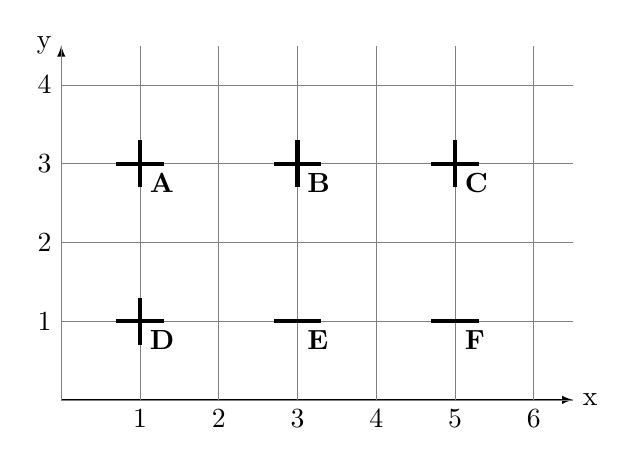
\begin{tikzpicture}
		\tikzstyle {point line} = [line width=0.15em]
				    
		\draw[-latex] (0,0) -- (6.5,0) node[right]{x};
		\draw[-latex] (0,0) -- (0,4.5) node[left]{y};
					
		\draw[help lines] (0,0) grid (6.5,4.5);
					
		\foreach \x in {1, 3, 5}
		\foreach \y in {1, 3}
		{
			\pgfmathsetmacro{\l}{\x - 0.3}
			\pgfmathsetmacro{\r}{\x + 0.3}
			                    
			\draw[point line] (\l,\y) -- (\r,\y);         
		}
		                
		\foreach \x in {1, 3, 5}
		{                    
			\draw[point line] (\x,3.3) -- (\x, 2.7);         
		}
		                
		\draw[point line] (1,1.3) -- (1, 0.7);     
				    
		\draw (1, 3) node [below right] {\textbf{A}};
		\draw (3, 3) node [below right] {\textbf{B}};
		\draw (5, 3) node [below right] {\textbf{C}};
		\draw (1, 1) node [below right] {\textbf{D}};
		\draw (3, 1) node [below right] {\textbf{E}};
		\draw (5, 1) node [below right] {\textbf{F}};	
				    
		\foreach \x in {1, 2, 3, 4, 5, 6}
		{
			\draw (\x, 0) node [below] {$\x$}	    ;
		}
				    
		\foreach \y in {1, 2, 3, 4}
		{
			\draw (0, \y) node [left] {$\y$}	    ;
		}
				    
	\end{tikzpicture}
	
\end{figure}

Following weak classifiers are considered. Their error points are shown below: 

\FloatBarrier
\begin{table}[htbp]
	\centering
	\begin{tabular}{|c|c|}
		\toprule
		\textbf{Weak Classifier} & \textbf{Error Points}  \\
		\midrule
		$x >= 2$                 & \textbf{A, D, E, F}    \\
		$x < 2$                  & \textbf{B, C}          \\
		$x >= 4$                 & \textbf{A, B, D, F}    \\
		$x < 4$                  & \textbf{C, E}          \\
		$x >= 6$                 & \textbf{A, B, C, D}    \\
		$x < 6$                  & \textbf{E, F}          \\
		$y >= 2$                 & \textbf{D}             \\
		$y < 2$                  & \textbf{A, B, C, E, F} \\
		$y >= 4$                 & \textbf{A, B, C, D}    \\
		$y < 4$                  & \textbf{E, F}          \\
		\hline
	\end{tabular}
\end{table}

\newcommand*\circled[1]{\tikz[baseline=(char.base)]{
	\node[shape=circle,draw,inner sep=2pt] (char) {#1};}}

\subsection{Iteration 1}
At the start, each point has an equal weight of $1/6$ since there are 6 points. 

\FloatBarrier
\begin{table}[htbp]
	\centering
	\begin{tabular}{|c|c|c|c|c|c|c|}
		\toprule
		\textbf{Point} & \textbf{A} & \textbf{B} & \textbf{C} & \textbf{D} & \textbf{E} & \textbf{F} \\
		\midrule
		\textbf{Error} & 1/6        & 1/6        & 1/6        & 1/6        & 1/6        & 1/6        \\
		\hline
	\end{tabular}
\end{table}
~\\

The error points and their corresponding weights determine the error rate of a particular weak classifier. The error rate for each classifier is shown below. 

\FloatBarrier \clearpage
\begin{table}[htbp]
	\centering
	\begin{tabular}{|c|c|}
		\toprule
		\textbf{Weak Classifier} & \textbf{Error Rate} \\
		\midrule
		$x >= 2$                 & 2/3                 \\
		$x < 2$                  & 1/3                 \\
		$x >= 4$                 & 2/3                 \\
		$x < 4$                  & 1/3                 \\
		$x >= 6$                 & 2/3                 \\
		$x < 6$                  & 1/3                 \\
		$y >= 2$                 & \circled{1/6}       \\
		$y < 2$                  & 5/6                 \\
		$y >= 4$                 & 2/3                 \\
		$y < 4$                  & 1/3                 \\
		\hline
	\end{tabular}
\end{table}

$y >= 2$ is chosen as the best weak classifier since it has the minimum error rate. $\alpha_1$ is calculated as follows: 
\begin{align*}
	\alpha_1 & = \frac{1}{2} \times ln(\frac{1-1/6}{1/6}) \\
	         & = \frac{1}{2} \times ln(5)                 
\end{align*}

\subsection{Iteration 2}
The weights are now updated as per flow chart above, 

\FloatBarrier
\begin{table}[htbp]
	\centering
	\begin{tabular}{|c|c|c|c|c|c|c|}
		\toprule
		\textbf{Point} & \textbf{A} & \textbf{B} & \textbf{C} & \textbf{D} & \textbf{E} & \textbf{F} \\
		\midrule
		\textbf{Error} & 1/10       & 1/10       & 1/10       & 1/2        & 1/10       & 1/10       \\
		\hline
	\end{tabular}
\end{table}

An interesting fact is that the sum of updated weights of the points misclassified by the chosen classifier $y >= 2$ (\textbf{D}) is equal to 1/2 and so the sum of updated weights of the points correctly classified (\textbf{A, B, C, E, F}) is also 1/2. 
\begin{align*}
	Error(\textbf{D})                                      & = 1/2                              \\
	\sum\limits_{P \in \{\textbf{A, B, C, E, F}\}}Error(P) & = 1/10 + 1/10 + 1/10 + 1/10 + 1/10 \\
	                                                       & = 1/2                              
\end{align*}

Error rates are updated as follows: 

\FloatBarrier\clearpage 
\begin{table}[htbp]
	\centering
	\begin{tabular}{|c|c|}
		\toprule
		\textbf{Weak Classifier} & \textbf{Error Rate} \\
		\midrule
		$x >= 2$                 & 4/5                 \\
		$x < 2$                  & \circled{1/5}       \\
		$x >= 4$                 & 4/5                 \\
		$x < 4$                  & 1/5                 \\
		$x >= 6$                 & 4/5                 \\
		$x < 6$                  & 1/5                 \\
		$y >= 2$                 & 1/2                 \\
		$y < 2$                  & 1/2                 \\
		$y >= 4$                 & 4/5                 \\
		$y < 4$                  & 1/5                 \\
		\hline
	\end{tabular}
\end{table}

$x < 2$ is chosen as the best weak classifier since it has the minimum error rate (for breaking tie, classifier occuring first in the above list is chosen).  
$\alpha_2$ is calculated as follows,
\begin{align*}
	\alpha_2 & = \frac{1}{2} \times ln(\frac{1-1/5}{1/5}) \\
	         & = \frac{1}{2} \times ln(4)                 
\end{align*}

\subsection{Iteration 3}

Weights are again updated as follows:

\FloatBarrier
\begin{table}[htbp]
	\centering
	\begin{tabular}{|c|c|c|c|c|c|c|}
		\toprule
		\textbf{Point} & \textbf{A} & \textbf{B} & \textbf{C} & \textbf{D} & \textbf{E} & \textbf{F} \\
		\midrule
		\textbf{Error} & 1/16       & 1/4        & 1/4        & 5/16       & 1/16       & 1/16       \\
		\hline
	\end{tabular}
\end{table}

Given that (\textbf{B, C}) are misclassified by $x<2$ and points (\textbf{A, D, E, F}) are correctly classified; notice again that,

\begin{align*}
	\sum\limits_{P \in \{\textbf{B, C}\}}Error(P)       & = 1/4 + 1/4                 \\
	                                                    & = 1/2                       \\
	\sum\limits_{P \in \{\textbf{A, D, E, F}\}}Error(P) & = 1/16 + 5/16 + 1/16 + 1/16 \\
	                                                    & = 1/2                       
\end{align*}

Updated error rates look like this,

\FloatBarrier\clearpage 
\begin{table}[htbp]
	\centering
	\begin{tabular}{|c|c|}
		\toprule
		\textbf{Weak Classifier} & \textbf{Error Rate} \\
		\midrule
		$x >= 2$                 & 1/2                 \\
		$x < 2$                  & 1/2                 \\
		$x >= 4$                 & 11/16               \\
		$x < 4$                  & 5/16                \\
		$x >= 6$                 & 7/8                 \\
		$x < 6$                  & \circled{1/8}       \\
		$y >= 2$                 & 5/16                \\
		$y < 2$                  & 11/16               \\
		$y >= 4$                 & 7/8                 \\
		$y < 4$                  & 1/8                 \\
		\hline
	\end{tabular}
\end{table}

$x < 6$ is chosen as the best weak classifier since it has the minimum error rate. 
$\alpha_3$ is calculated as follows,
\begin{align*}
	\alpha_3 & = \frac{1}{2} \times ln(\frac{1-1/8}{1/8}) \\
	         & = \frac{1}{2} \times ln(7)                 
\end{align*}

After three iterations, the resultant strong classifier is 

\begin{align*}
	H = & sign(\frac{1}{2} \times ln(5) \times (y>=2) \\ 
	    & + \frac{1}{2} \times ln(4) \times (x<2)     \\ 
	    & + \frac{1}{2} \times ln(7) \times (x<6) )   
\end{align*}

The classification of $H$ for each point is as follows,

\FloatBarrier
\begin{table}[htbp]
	\centering
	\begin{tabular}{|c|c|c|}
		\toprule
		\textbf{Point}   & \textbf{Calculation}                      & \textbf{Classification} \\
		\midrule
		\rule{0pt}{1ex}A & $sign(1/2 \times ln(5\times 4 \times 7))$ & $+$                     \\
		\rule{0pt}{1ex}B & $sign(1/2 \times ln((5 \times 7) / 4))$   & $+$                     \\
		\rule{0pt}{1ex}C & $sign(1/2 \times ln((5 \times 7) / 4))$   & $+$                     \\
		\rule{0pt}{1ex}D & $sign(1/2 \times ln((4 \times 7) / 5))$   & $+$                     \\
		\rule{0pt}{1ex}E & $sign(1/2 \times ln(7 / (5 \times 4)))$   & $-$                     \\
		\rule{0pt}{1ex}F & $sign(1/2 \times ln(7 / (5 \times 4)))$   & $-$                     \\        
		\hline
	\end{tabular}
\end{table}

It is evident the $H$ classifies each point correctly after 3 iterations. Further iterations are hence terminated.

\section{Mathematics}

\subsection{Upper bound on training error}
\subsubsection{Step 1}

\begin{align*}
	Error(H_T) = \frac{1}{N} \times \sum\limits_{i} \left\{ 
	\begin{array}{ll}                                       
	1 \text{\ if\ } y_i \neq H_T(x_i)                       \\
	0 \text{\ else}                                         
	\end{array}                                             
	\right.                                                 
\end{align*}

Let $H_T(x_i) = sign(f_T(x_i))$ where $f_T(x_i) = \sum\limits_{t}\alpha_t \times h_t(x_i)$

\begin{align*}
	Error(H_T) = \frac{1}{N} \times \sum\limits_{i} \left\{ 
	\begin{array}{ll}                                       
	1 \text{\ if\ } y_i \times f_T(x_i) <= 0                \\
	0 \text{\ else}                                         
	\end{array}                                             
	\right.                                                 
\end{align*}

\FloatBarrier
\begin{figure}[htbp]
	\centering
	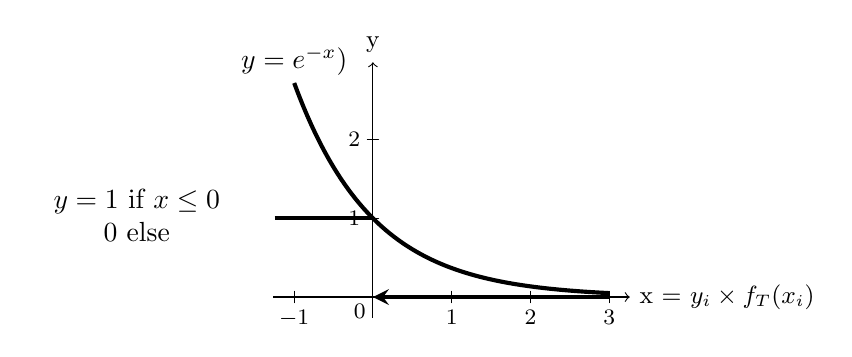
\begin{tikzpicture}
		\datavisualization [school book axes,
			visualize as smooth line/.list={func},
			func={style={line width=0.15em}},
			y axis={label={y}},
		x axis={label={x = $y_i \times f_T(x_i)$}} ]
					
		data [set=func, format=function] {
			var x : interval [-1:3] samples 100;
			func y = e^(-\value{x});
		};
		\draw [line width=0.15em] (-1.25, 1) -- (0, 1);
		\draw [line width=0.15em, <-, >=stealth] (0, 0) -- (3, 0);
		    
		\node at (-3, 1) {\begin{tabular}{c}
			$y = 1\ \text{if}\ x \leq 0$ \\
			$0\ \text{else}$ 
			\end{tabular}}; 
		\node at (-1, 3) {$y=e^{-x})$}; 
	\end{tikzpicture}
\end{figure}

\begin{align}
	Error(H_T) \leq \frac{1}{N} \times \sum\limits_{i} e^{-y_i \times f_T(x_i)} 
\end{align}

\subsubsection{Step 2}

\begin{align*}
	w_{t+1}(i) = \frac{1}{2} \times w_t(i) \left\{      
	\begin{array}{ll}                                   
	\frac{1}{1-\epsilon_{t}}\ \text{if}\ y_i = h_t(x_i) \\
	\frac{1}{\epsilon_{t}}\ \ \ \ \text{else}           \\
	\end{array}                                         
	\right.                                             
\end{align*}

\begin{align*}
	w_{t+1}(i) = \frac{w_t(i)}{2\times \sqrt[]{\epsilon_t \times (1- \epsilon_t)}} \left\{ 
	\begin{array}{ll}                                                                      
	\sqrt[]{\frac{\epsilon_t}{1-\epsilon_t}}\ \text{if}\ y_i = h_t(x_i)                    \\
	\sqrt[]{\frac{1-\epsilon_t}{\epsilon_t}}\ \text{else}                                  \\
	\end{array}                                                                            
	\right.                                                                                
\end{align*}

\begin{align*}
	w_{t+1}(i) = \frac{w_t(i)}{2\times \sqrt[]{\epsilon_t \times (1- \epsilon_t)}} \times e^{-\alpha_t \times y_i \times h_t(x_i)} 
\end{align*}

\begin{align*}
	w_{t+1}(i) = \frac{1}{2\times \prod\limits_t{\sqrt[]{\epsilon_t \times (1- \epsilon_t}})} \times e^{-y_i \times f_t(x_i)} \times \frac{1}{N} 
\end{align*}

Transposing and replacing $t$ by $T$,

\begin{align*}
	\frac{1}{N} \times e^{-y_i \times f_T(x_i)}  = 2 \times w_{T+1}(i) \times \prod\limits_t{\sqrt[]{\epsilon_t \times (1- \epsilon_t}}) 
\end{align*}

Summing over i,

\begin{align*}
	\sum\limits_i \frac{1}{N} \times e^{-y_i \times f_T(x_i)}  = 2 \times \prod\limits_t{\sqrt[]{\epsilon_t \times (1- \epsilon_t}}) \times \sum\limits_i w_{T+1}(i) 
\end{align*}

Since sum of weights is one at every round,

\begin{align}
	\frac{1}{N} \times \sum\limits_i  e^{-y_i \times f_T(x_i)}  = 2 \times \prod\limits_t{\sqrt[]{\epsilon_t \times (1- \epsilon_t}}) 
\end{align}

\subsubsection{Step 3}

Using (1) and (2)

\begin{align*}
	Error(H_T) \leq 2 \times \prod\limits_t{\sqrt[]{\epsilon_t \times (1- \epsilon_t}}) 
\end{align*}

Using $\gamma_t = (1/2 - \epsilon_t)$

\begin{align*}
	Error(H_T) \leq 2 \times \prod\limits_t{\sqrt[]{1/4 - \gamma_t^2}} 
\end{align*}

\begin{align*}
	Error(H_T) \leq \prod\limits_t{\sqrt[]{1 - 4\gamma_t^2}} 
\end{align*}

Since $e^x \geq (1+x)$ for all real values of $x$,

\begin{align*}
	Error(H_T) \leq \prod\limits_t{e^{-2\gamma_t^2}} 
\end{align*}

\begin{align*}
	Error(H_T) \leq e^{-2\sum\limits_t{\gamma_t^2}} 
\end{align*}

Since $\sum\limits_t{\gamma_t^2}$ monotonically increases with each iteration, $Error(H_t)$ monotonically decreases exponentially.


\end{document}